\subsection{Web Application Programming Interfaces}

This section gives an overview over the basic concepts and technologies behind Web \acp{API}.

\subsubsection{Use Cases and Types of Web APIs}

An \ac{API} in general is an interface between two pieces of software\cite[S.1]{reddy2011api}.
It abstracts complex functionality away and provides a simple interface
to interact with to retrieve data and services\cite{Mozilla}.
Web APIs are a specific form of API that can be accessed over the internet
using the HTTP protocol.\cite{StoplightAPITypes}
They are used to power desktop, web and mobile applications. pass data between different
services, systems and devices. They make automated data access and retrieval possible
and enable the integration of internal and external systems into processes and data flows.\cite{Lane2019WhatIs}

There are different types of Web APIs, mainly Open/Public APIs, Internal APIs and Partner APIs\cite{StoplightAPITypes}.
Open APIs are provided by a company, government or other organization and make it possible for any developer
to access that organizations data or services\cite{StoplightAPITypes}.
Internal APIs are only used to share resources within one organization, while
partner APIs are exposed to the public, but are only open to specific users, which might pay for
the right to use the API\cite{StoplightAPITypes}.

Spotify offers a Public Web API, which is used in this project in the context of data collection (section \ref{sec:Data Collection}).
In order to understand the specifics of data collection,
some concepts regarding the \ac{HTTP} protocol are explained in the following section.

\subsubsection{The HTTP Protocol}

All communication on the world wide web is conducted through \ac{HTTP}
because of its reliability and guarantee for data integrity\cite[3f.]{gourley2002http}.

Most communication on the Web is conducted between a client and a server. The client usually
requests a resource from the server and the server responds with that resource, which the client
can then use\cite[4]{gourley2002http}.


To tell the server, which specific resource it wants, the client uses a \ac{URL}, which 
uniquely identifies a resource on the web. 
Figure \ref{fig:Description of different parts of a URL} shows how URLs are structured.
If the server knows where to find the resource and the client is authorized to see it,
the server will send it to the client.
In the context of APIs, a URL pointing to a specific resource is also called an "API endpoint".\cite{Cooksey2014}
This interaction between client and server is usually done in an HTTP transaction.

\begin{figure}[H]
    \caption{Description of different parts of a URL}
	\label{fig:Description of different parts of a URL}
    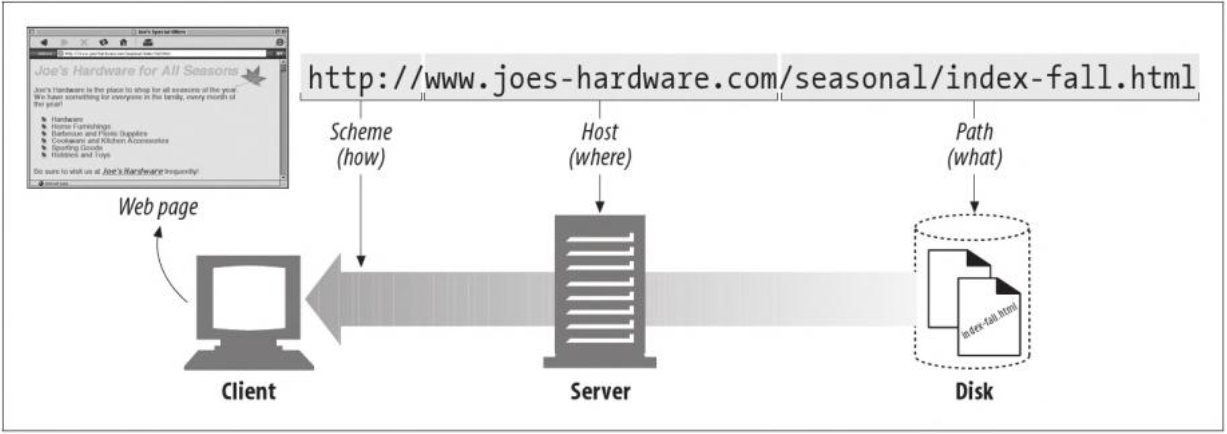
\includegraphics[width=1\textwidth]{URLDescription}
    \\
    Source: \cite[24]{gourley2002http}
\end{figure}

A transaction consists of a request (sent from client to server) and a response in which the
server answers the clients request in some way.\cite[8]{gourley2002http}
In the context of Web APIs, a request made to an API is also called "API call".\cite{StoplightAPITypes}
Figure \ref{fig:Example HTTP request and response messages} shows the structure of an 
HTTP request and response message.

\begin{figure}[H]
    \caption{Example HTTP request and response messages}
	\label{fig:Example HTTP request and response messages}
    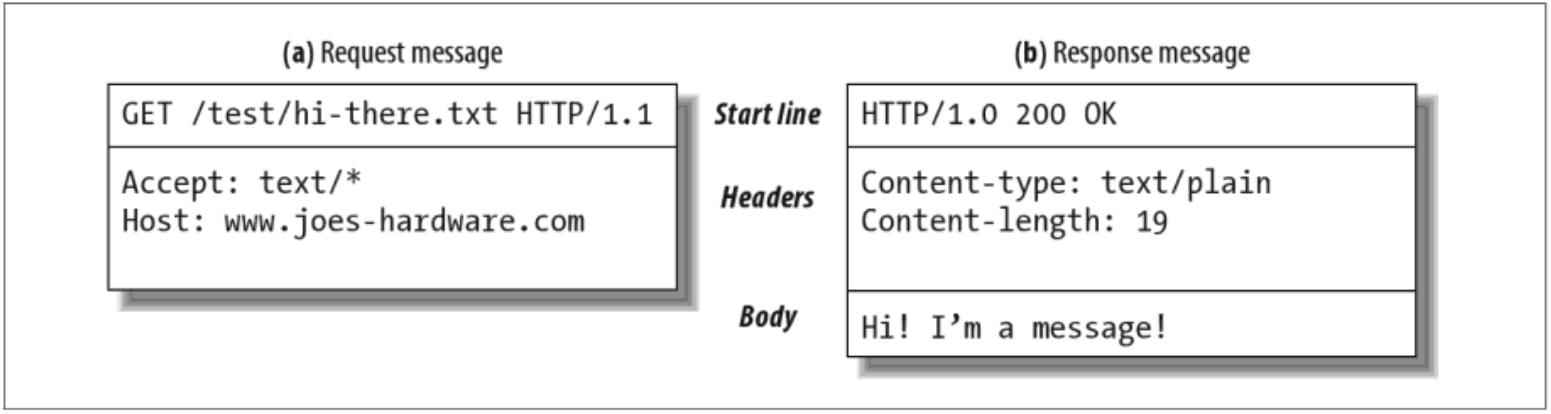
\includegraphics[width=1\textwidth]{HTTPMessageExample}
    \\
    Source: \cite[47]{gourley2002http}
\end{figure}

Every HTTP request message starts with a method.
There are many HTTP methods defined, that can be used to delete a resource, store
data on the server, get header information for a document and more.\cite[48]{gourley2002http}
In this paper, only two HTTP methods are used, GET and POST.
A GET request is used to ask the server to send a resource to the client.
It does not contain a body.\cite[48]{gourley2002http}
A POST request message is used to send data to the server for processing. The data to be
processed is sent in the request body.\cite[48]{gourley2002http}

A request also includes the URL, protocol information and a set of headers, delivering
additional information about the client \cite[47]{gourley2002http}.

Response messages contain a status code instead of a method or URL.


Every HTTP request message has a start line.
It contains a method, which tells the server what action to perform on the resource, the URL
and some protocol information.\cite[47]{gourley2002http}
After the start line, some headers are given. These contain information about the request,
e.g. what types of data the client can accept or credentials for authorization.
Some requests also contain a body to give some data to the server. \cite[52]{gourley2002http}

A response message does not contain a method or URL
Instead it contains protocol information and status information in the form of a numerical
status code and status text.\cite[48]{gourley2002http}
A response also contains headers and might contain a body.\cite[52]{gourley2002http}

Status codes tell the client if the transaction was successful or what type of problem occured\cite[49]{gourley2002http}.
%Some possible status might be success, the server not being able to find a resource, not
%being able to store the data, or the client being unauthorized to see the data\\
There are many status codes defined in the HTTP standard,
some of the most common ones are shown in table \ref{tbl:Common status codes}.

\begin{table}[H]
 \caption{Common status codes}
 \label{tbl:Common status codes}
\begin{tabular}{|| c | c | c ||} 
 \hline
 Status code & Reason phrase & Meaning \\ [0.5ex]
 \hline\hline
 200 & OK & Successful transaction. Any requested data is in the response body \\ [1ex]
 \hline
 401 & Unauthorized & The response needs to contain credentials to access the requested resource. \\ [1ex]
 \hline
 404 & Not Found & The server cannot find a resource for the requested URL. \\ [1ex]
 \hline
\end{tabular}
Source: \cite[50]{gourley2002http}
\end{table}


%There are many HTTP methods defined, that can be used to delete a resource, store
%data on the server, get header information for a document and more.\cite[48]{gourley2002http}
%In this paper, only two HTTP methods are used, GET and POST.
%A GET request is used to ask the server to send a resource to the client.
%It does not contain a body.\cite[48]{gourley2002http}
%A POST request message is used to send data to the server for processing. The data to be
%processed is sent in the request body.\cite[48]{gourley2002http}


\subsubsection{JSON}

The Spotify API uses the \ac{JSON} data format to transfer data to the client\cite{SpotifyWebAPI}.

Most modern APIs transmit data to the client using \ac{JSON}.
It is a text-based format able to represent semi-structured data. \cite{MozillaJSON}
JSON objects are simple, have good readability and are easily processed by computers,
which explains the wide usage of the data format\cite{OracleJSON}.
JSON is tightly integrated in the JavaScript programming language and can be used without any parsing or serialization.\cite{OracleJSON}
This is beneficial, as JavaScript is widely used both on the client and server side of web applications. 
JSON can also be used with many other programming languages. \cite{JsonOrgIntroduction}

JSON supports only six very basic datatypes: String, Number, Boolean, Null, Object and Array.\cite{OracleJSON}
The following code snippet shows how each of the datatypes are defined in JSON.

\begin{lstlisting}[language=JavaScript]
    {
        "string": "Martin",
        "number": 200,
        "number2": 300,
        "boolean": true,
        "booleanFalse": false,
        "nullValue": null,
        "object": {
            "objectAttribute": "string",
            "objectAttribute2": "string2"
        },
        "array": [
            "entry1",
            "entry2",
            {
                "objectInArray": true
            }
        ]
    }
\end{lstlisting}

The code snippet shows, that the whole JSON object is wrapped in curly braces.
Each attribute is defined as an attribute-value-pair, where the attribute name is defined in 
double quotes, followed by a colon and the value definition. String values are defined in 
double quotes, numbers and booleans without. Objects are defined in curly braces and can
again contain any datatype.
Arrays are defined using brackets. They can contain any number of entries of any type.
Types can also be mixed within the same array.
All attributes-value-pairs or array items are seperated by commas.
Indentation and newline characters are not parsed in JSON as all syntax is given using
the characters '"{}[]:,'.\cite{JsonOrgIntroduction}

%\subsubsection{The REST Architecture}
%
%\ac{REST} is a set of constraints applied to modern web services, that stems from a basic set
%of rules, which were defined to ensure the scalability of the web.\cite[5]{masse2011rest}
%A web service, which implements REST principles is also called a "RESTful service".
%Such an API consists of a set of interlinked resources called a resource model.\cite[6]{masse2011rest}
%
%There are six basic rules to a RESTful design:\cite[2]{masse2011rest}
%\begin{itemize}
%    \item Client-server: The API is designed to work in a client/server architecture.\cite[3]{masse2011rest}
%    \item Uniform Interface: The API needs to conform to the established standards of the web.\cite[3]{masse2011rest}
%    This includes
%    \begin{itemize}
%        \item Identification of resources through a unique identifier, such as a URL.\cite[3]{masse2011rest}
%        \item The manipulation of resources through representations.
%        This means that information about the resource is only exchanged using representations.
%        As an example, a set of data could be stored in a database on the server. When a client
%        requests the resource, a JSON representation of the data is sent, not the actual database.
%        This ensures flexibility and interoperability, as the data could also be represented using
%        other models, such as XML.\cite[3]{masse2011rest}
%        \item Self-discriptive messages, which means that a HTTP message should always completely
%        describe the action to be performed on the server. No additional knowledge or state should
%        be required to understand the message.\cite[3]{masse2011rest}
%        \item Hypermedia as the engine of application state. This means that links to other
%        resources can be used in a resource's representation to describe its state or the state of
%        other resources.\cite[3]{masse2011rest}
%    \end{itemize}
%    \item Layered System: This enables the use of proxies, gateways to
%    enforce security balance server load.\cite[3]{masse2011rest}
%    \item Cache: The response from a web server should always include information about the
%    cacheability of the response data. This ensures load reduction, availability and low latency.\cite[3]{masse2011rest}
%    \item Stateless: A web server must not be required to save information about the state,
%    which the client receiving the data is in. Clients should always communicate their state to
%    the server so it can respond accordingly.\cite[3]{masse2011rest}
%    \item Code-On-Demand: This means that servers must be able to transfer the execution of code to the client,
%    e.g. in the form of client-side JavaScript.\cite[3]{masse2011rest}
%\end{itemize}
%
%All RESTful APIs should follow these rules and users of the API can expect it to handle
%resources and state in this way.